\documentclass[]{article}
\usepackage{lmodern}
\usepackage{amssymb,amsmath}
\usepackage{ifxetex,ifluatex}
\usepackage{fixltx2e} % provides \textsubscript
\ifnum 0\ifxetex 1\fi\ifluatex 1\fi=0 % if pdftex
  \usepackage[T1]{fontenc}
  \usepackage[utf8]{inputenc}
\else % if luatex or xelatex
  \ifxetex
    \usepackage{mathspec}
  \else
    \usepackage{fontspec}
  \fi
  \defaultfontfeatures{Ligatures=TeX,Scale=MatchLowercase}
\fi
% use upquote if available, for straight quotes in verbatim environments
\IfFileExists{upquote.sty}{\usepackage{upquote}}{}
% use microtype if available
\IfFileExists{microtype.sty}{%
\usepackage{microtype}
\UseMicrotypeSet[protrusion]{basicmath} % disable protrusion for tt fonts
}{}
\usepackage[margin=1in]{geometry}
\usepackage{hyperref}
\hypersetup{unicode=true,
            pdftitle={Breve Introducción a R},
            pdfauthor={Juan Carlos Castillo},
            pdfborder={0 0 0},
            breaklinks=true}
\urlstyle{same}  % don't use monospace font for urls
\usepackage{color}
\usepackage{fancyvrb}
\newcommand{\VerbBar}{|}
\newcommand{\VERB}{\Verb[commandchars=\\\{\}]}
\DefineVerbatimEnvironment{Highlighting}{Verbatim}{commandchars=\\\{\}}
% Add ',fontsize=\small' for more characters per line
\usepackage{framed}
\definecolor{shadecolor}{RGB}{248,248,248}
\newenvironment{Shaded}{\begin{snugshade}}{\end{snugshade}}
\newcommand{\AlertTok}[1]{\textcolor[rgb]{0.94,0.16,0.16}{#1}}
\newcommand{\AnnotationTok}[1]{\textcolor[rgb]{0.56,0.35,0.01}{\textbf{\textit{#1}}}}
\newcommand{\AttributeTok}[1]{\textcolor[rgb]{0.77,0.63,0.00}{#1}}
\newcommand{\BaseNTok}[1]{\textcolor[rgb]{0.00,0.00,0.81}{#1}}
\newcommand{\BuiltInTok}[1]{#1}
\newcommand{\CharTok}[1]{\textcolor[rgb]{0.31,0.60,0.02}{#1}}
\newcommand{\CommentTok}[1]{\textcolor[rgb]{0.56,0.35,0.01}{\textit{#1}}}
\newcommand{\CommentVarTok}[1]{\textcolor[rgb]{0.56,0.35,0.01}{\textbf{\textit{#1}}}}
\newcommand{\ConstantTok}[1]{\textcolor[rgb]{0.00,0.00,0.00}{#1}}
\newcommand{\ControlFlowTok}[1]{\textcolor[rgb]{0.13,0.29,0.53}{\textbf{#1}}}
\newcommand{\DataTypeTok}[1]{\textcolor[rgb]{0.13,0.29,0.53}{#1}}
\newcommand{\DecValTok}[1]{\textcolor[rgb]{0.00,0.00,0.81}{#1}}
\newcommand{\DocumentationTok}[1]{\textcolor[rgb]{0.56,0.35,0.01}{\textbf{\textit{#1}}}}
\newcommand{\ErrorTok}[1]{\textcolor[rgb]{0.64,0.00,0.00}{\textbf{#1}}}
\newcommand{\ExtensionTok}[1]{#1}
\newcommand{\FloatTok}[1]{\textcolor[rgb]{0.00,0.00,0.81}{#1}}
\newcommand{\FunctionTok}[1]{\textcolor[rgb]{0.00,0.00,0.00}{#1}}
\newcommand{\ImportTok}[1]{#1}
\newcommand{\InformationTok}[1]{\textcolor[rgb]{0.56,0.35,0.01}{\textbf{\textit{#1}}}}
\newcommand{\KeywordTok}[1]{\textcolor[rgb]{0.13,0.29,0.53}{\textbf{#1}}}
\newcommand{\NormalTok}[1]{#1}
\newcommand{\OperatorTok}[1]{\textcolor[rgb]{0.81,0.36,0.00}{\textbf{#1}}}
\newcommand{\OtherTok}[1]{\textcolor[rgb]{0.56,0.35,0.01}{#1}}
\newcommand{\PreprocessorTok}[1]{\textcolor[rgb]{0.56,0.35,0.01}{\textit{#1}}}
\newcommand{\RegionMarkerTok}[1]{#1}
\newcommand{\SpecialCharTok}[1]{\textcolor[rgb]{0.00,0.00,0.00}{#1}}
\newcommand{\SpecialStringTok}[1]{\textcolor[rgb]{0.31,0.60,0.02}{#1}}
\newcommand{\StringTok}[1]{\textcolor[rgb]{0.31,0.60,0.02}{#1}}
\newcommand{\VariableTok}[1]{\textcolor[rgb]{0.00,0.00,0.00}{#1}}
\newcommand{\VerbatimStringTok}[1]{\textcolor[rgb]{0.31,0.60,0.02}{#1}}
\newcommand{\WarningTok}[1]{\textcolor[rgb]{0.56,0.35,0.01}{\textbf{\textit{#1}}}}
\usepackage{graphicx,grffile}
\makeatletter
\def\maxwidth{\ifdim\Gin@nat@width>\linewidth\linewidth\else\Gin@nat@width\fi}
\def\maxheight{\ifdim\Gin@nat@height>\textheight\textheight\else\Gin@nat@height\fi}
\makeatother
% Scale images if necessary, so that they will not overflow the page
% margins by default, and it is still possible to overwrite the defaults
% using explicit options in \includegraphics[width, height, ...]{}
\setkeys{Gin}{width=\maxwidth,height=\maxheight,keepaspectratio}
\IfFileExists{parskip.sty}{%
\usepackage{parskip}
}{% else
\setlength{\parindent}{0pt}
\setlength{\parskip}{6pt plus 2pt minus 1pt}
}
\setlength{\emergencystretch}{3em}  % prevent overfull lines
\providecommand{\tightlist}{%
  \setlength{\itemsep}{0pt}\setlength{\parskip}{0pt}}
\setcounter{secnumdepth}{0}
% Redefines (sub)paragraphs to behave more like sections
\ifx\paragraph\undefined\else
\let\oldparagraph\paragraph
\renewcommand{\paragraph}[1]{\oldparagraph{#1}\mbox{}}
\fi
\ifx\subparagraph\undefined\else
\let\oldsubparagraph\subparagraph
\renewcommand{\subparagraph}[1]{\oldsubparagraph{#1}\mbox{}}
\fi

%%% Use protect on footnotes to avoid problems with footnotes in titles
\let\rmarkdownfootnote\footnote%
\def\footnote{\protect\rmarkdownfootnote}

%%% Change title format to be more compact
\usepackage{titling}

% Create subtitle command for use in maketitle
\providecommand{\subtitle}[1]{
  \posttitle{
    \begin{center}\large#1\end{center}
    }
}

\setlength{\droptitle}{-2em}

  \title{Breve Introducción a R}
    \pretitle{\vspace{\droptitle}\centering\huge}
  \posttitle{\par}
    \author{Juan Carlos Castillo}
    \preauthor{\centering\large\emph}
  \postauthor{\par}
    \date{}
    \predate{}\postdate{}
  

\begin{document}
\maketitle

\hypertarget{notas-introductorias}{%
\subsection{Notas introductorias}\label{notas-introductorias}}

\begin{itemize}
\tightlist
\item
  R Corresponde más a un marco de análisis estadístico que a un programa
  estadístico, con una fuerte orientación a ciencia de datos (Data
  Science)
\item
  Gratuito y de código abierto
\item
  Actualmente se combina con una serie de herramientas de ciencia de
  datos para facilitar reportes y reproducibilidad de los análisis
\item
  El registro de los análisis queda en formato de texto plano, por lo
  tanto es independiente de una plataforma para poder editarlo, y además
  permite un control eficiente de versiones (por ejemplo vía Git).
\item
  Los análisis operan en base a paquetes o librerias
\item
  Actualmente existen más de 3000 librerías disponibles
\item
  Particularidad: el análisis se orienta a objetos (detalle más
  adelante)
\end{itemize}

\hypertarget{instalacion-r-rstudio}{%
\subsection{1. Instalación R / Rstudio}\label{instalacion-r-rstudio}}

\begin{itemize}
\item
  Visitar la página de CRAN (Comprehensive R Archive Network),
  \url{http://cran.r-project.org/}
\item
  Seleccionar versión según sistema operativo (Ej. Linux)
\item
  Instalar ``base''
\item
  En el caso de Windows, el programa R GUI (Graphical User Interface)se
  agrega a la lista de programas y apareceicono de acceso desde
  elescritorio. Es la interfaz de R por defecto
\item
  Nota: Existen otras interfaces gráficas (GUIs) para trabajar con R,
  como Commander o Java GUI for R (Jaguar), Deducer, R-Studio, etc.
\item
  Interfaz recomendada: R Studio,\url{https://www.rstudio.com/}
\item
  Actualización:

  \begin{itemize}
  \tightlist
  \item
    Bajar e instalar nueva versión
  \item
    Copiar librerías de carpeta antigua a la nueva
  \item
    Actualizar librerías (update packages)
  \end{itemize}
\end{itemize}

\hypertarget{trabajando-en-r}{%
\subsection{2. Trabajando en R}\label{trabajando-en-r}}

\hypertarget{bases}{%
\subsubsection{Bases}\label{bases}}

\begin{itemize}
\tightlist
\item
  RStudio posee 4 ventanas (panes): las dos principales son el editor
  (source) y consola; las otras dos tienen relación con entorno,
  paquetes, plots, etc.
\item
  El orden como se presentan estas cuatro ``panes'' se puede cambiar en
  Tools/Options/Pane Layout
\item
  Se pueden ingresar comandos directamente en la consola, por ejemplo:
\end{itemize}

\begin{Shaded}
\begin{Highlighting}[]
\DecValTok{4}\OperatorTok{+}\DecValTok{1}
\DecValTok{4}\OperatorTok{>}\DecValTok{1}
\end{Highlighting}
\end{Shaded}

\begin{itemize}
\tightlist
\item
  Los comandos se escriben en el prompt \texttt{(\textgreater{})}, y se
  ejecutan con la tecla \textbf{enter}
\item
  El número entre paréntesis cuadrado (ej. {[}1{]}) indica el orden de
  aparición de los resultados
\item
  Sin embargo, la manera habitual de trabajar es de un archivo de
  código, donde quedan registrados los comandos (análogo a do file de
  Stata)
\item
  También existen algunas opciones de menú, las que tienen relación con
  edición y la configuración del programa (no con el análisis de datos)
\item
  Para salir de R , cerrar ventana o ejecutar \texttt{q()}
\end{itemize}

\hypertarget{trabajando-desde-un-archivo-de-codigo-script}{%
\subsubsection{Trabajando desde un archivo de código
(script)}\label{trabajando-desde-un-archivo-de-codigo-script}}

\begin{itemize}
\tightlist
\item
  File - new script
\item
  Archivo en que se ingresan los comandos correspondientes a un análisis
  específico, los cuales pueden ser guardados y ejecutados
  posteriormente
\item
  Para correr los comandos desde el editor, posicionar el cursor en la
  línea respectiva y luego ``ctrl r'' o ``F5'', o con elicono de
  ejecución
\item
  Para grabar scripts: File - save as
\item
  Por defecto graba con extensión .R, pero es sólo un archivo de formato
  simple (txt) que se puede abrir con cualquier editor de texto (ej.
  Block de notas).
\item
  Para abrir script grabado: File - open script
\item
  Caracteres especiales
\end{itemize}

\begin{verbatim}
# Comentarios (AltGr 3) , no se ejecutan
+ Sigue el comando en la próxima linea
; Para escribir más de una función en la misma línea de comandos
\end{verbatim}

\hypertarget{librerias}{%
\subsubsection{Librerías}\label{librerias}}

\begin{itemize}
\tightlist
\item
  Conjunto de funciones que tienen una relación entre ellas y que
  usualmente vienen acompañadas de ficheros de ayuda (documentación)
\item
  Algunas librerías vienen preinstaladas, otras específicas hay que
  instalarlas de acuerdo a las necesidades del usuario
\item
  Para conocer la lista de librerías instaladas: \texttt{library()}
\item
  Para instalar: \texttt{install.packages(librería)}, en el caso que se
  sepa el nombre específico de la librería que se quiera instalar. O
  mediante menú : Packages - Install package(s)
\item
  Las librerías se instalan sólo 1 vez y quedan guardadas en una carpeta
  local, pero deben ser cargadas si se quieren utilizar en la sesión de
  trabajo con \texttt{library("library”)}
\item
  Para explorar librerías disponibles: \url{http://cran.r-project.org/},
  organizadas por área en Task Views
\item
  Ej: instalar librería psy
\end{itemize}

\begin{Shaded}
\begin{Highlighting}[]
\KeywordTok{install.packages}\NormalTok{(}\StringTok{"psy"}\NormalTok{)}
\KeywordTok{library}\NormalTok{(psy)}
\NormalTok{? psy }\CommentTok{# Ayuda de la libreria}
\end{Highlighting}
\end{Shaded}

\textbf{Instalación/carga de librerías con \texttt{pacman}}

\begin{itemize}
\item
  Para evitar el tener que instalar/cargar librerías, la mejor solución
  es utilizar la librería \texttt{pacman}
\item
  Se instala, y luego en las siguientes sesiones se utiliza el siguiente
  código con las librerías a utilizar (por ejemplo, lavaan)
\end{itemize}

\begin{Shaded}
\begin{Highlighting}[]
\CommentTok{# install.packages("pacman") # solo la primera vez}
\NormalTok{pacman}\OperatorTok{::}\KeywordTok{p_load}\NormalTok{(lme4)}
\end{Highlighting}
\end{Shaded}

\begin{itemize}
\tightlist
\item
  Si la librería está instalada, solo la carga; si no, la instala y la
  carga.
\end{itemize}

\hypertarget{objetos}{%
\subsubsection{Objetos}\label{objetos}}

\begin{itemize}
\item
  R es un programa orientado a objetos, los que son creados por
  funciones, que en su forma más general sería:
  \texttt{Objeto\ \textless{}-\ función} o de manera equivalente
  \texttt{Objeto\ =\ función}
\item
  Diferentes tipos de objetos: vectores, factores, matrices, marco/base
  de datos (entre otros)
\item
  Objetos simples:
\end{itemize}

\begin{Shaded}
\begin{Highlighting}[]
\NormalTok{x =}\StringTok{ }\DecValTok{5} \CommentTok{# el número 5 es asignado al objeto x}
\NormalTok{x}
\end{Highlighting}
\end{Shaded}

\begin{verbatim}
## [1] 5
\end{verbatim}

\begin{Shaded}
\begin{Highlighting}[]
\CommentTok{## [1] 5}
\NormalTok{a =}\StringTok{ "hoy"}
\NormalTok{a}
\end{Highlighting}
\end{Shaded}

\begin{verbatim}
## [1] "hoy"
\end{verbatim}

\begin{Shaded}
\begin{Highlighting}[]
\CommentTok{## [1] "hoy"}
\end{Highlighting}
\end{Shaded}

\textbf{Vectores}

\begin{itemize}
\tightlist
\item
  Objeto unidimensional constituido por elementos del mismo tipo
\end{itemize}

\begin{Shaded}
\begin{Highlighting}[]
\NormalTok{edad =}\StringTok{ }\KeywordTok{c}\NormalTok{(}\DecValTok{50}\NormalTok{,}\DecValTok{1}\NormalTok{,}\DecValTok{25}\NormalTok{,}\DecValTok{6}\NormalTok{) }\CommentTok{# c es por "concatenate"}
\NormalTok{edad}
\end{Highlighting}
\end{Shaded}

\begin{verbatim}
## [1] 50  1 25  6
\end{verbatim}

\begin{Shaded}
\begin{Highlighting}[]
\NormalTok{alumnos =}\StringTok{ }\KeywordTok{c}\NormalTok{(}\StringTok{"juan"}\NormalTok{, }\StringTok{"simón", "}\NormalTok{maría}\StringTok{", "}\NormalTok{sonia}\StringTok{")}
\StringTok{alumnos}
\end{Highlighting}
\end{Shaded}

\begin{verbatim}
## [1] "juan"  "simón" "maría" "sonia"
\end{verbatim}

\begin{Shaded}
\begin{Highlighting}[]
\NormalTok{hasta20 =}\StringTok{ }\DecValTok{1}\OperatorTok{:}\DecValTok{20} \CommentTok{#genera una secuencia de números del 1 al 20}
\NormalTok{hasta20}
\end{Highlighting}
\end{Shaded}

\begin{verbatim}
##  [1]  1  2  3  4  5  6  7  8  9 10 11 12 13 14 15 16 17 18 19 20
\end{verbatim}

\begin{Shaded}
\begin{Highlighting}[]
\NormalTok{a =}\StringTok{ }\KeywordTok{seq}\NormalTok{ (}\DataTypeTok{from =} \DecValTok{-5}\NormalTok{, }\DataTypeTok{to =} \DecValTok{5}\NormalTok{, }\DataTypeTok{by =} \FloatTok{1.5}\NormalTok{)}
\NormalTok{a}
\end{Highlighting}
\end{Shaded}

\begin{verbatim}
## [1] -5.0 -3.5 -2.0 -0.5  1.0  2.5  4.0
\end{verbatim}

\begin{Shaded}
\begin{Highlighting}[]
\NormalTok{tresdos =}\StringTok{ }\KeywordTok{rep}\NormalTok{(}\DecValTok{2}\NormalTok{,}\DecValTok{3}\NormalTok{)}
\NormalTok{tresdos}
\end{Highlighting}
\end{Shaded}

\begin{verbatim}
## [1] 2 2 2
\end{verbatim}

\begin{verbatim}
Ejemplo de operaciones con vectores numéricos
\end{verbatim}

\begin{Shaded}
\begin{Highlighting}[]
\KeywordTok{mean}\NormalTok{(edad)}
\end{Highlighting}
\end{Shaded}

\begin{verbatim}
## [1] 20.5
\end{verbatim}

\begin{Shaded}
\begin{Highlighting}[]
\KeywordTok{summary}\NormalTok{(edad)}
\end{Highlighting}
\end{Shaded}

\begin{verbatim}
##    Min. 1st Qu.  Median    Mean 3rd Qu.    Max. 
##    1.00    4.75   15.50   20.50   31.25   50.00
\end{verbatim}

\emph{Algunas otras funciones}

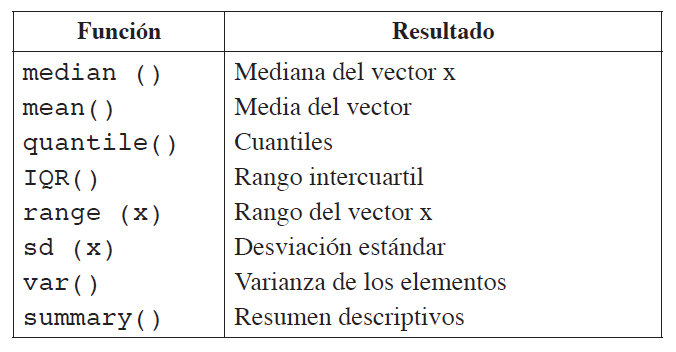
\includegraphics[width=0.7\textwidth,height=\textheight]{vectorfunc.jpg}

\textbf{Factores}

\begin{itemize}
\tightlist
\item
  Modo que utiliza R para almacenar variables categóricas
\end{itemize}

\begin{Shaded}
\begin{Highlighting}[]
\NormalTok{sexo <-}\StringTok{ }\KeywordTok{c}\NormalTok{(}\KeywordTok{rep}\NormalTok{(}\StringTok{"mujer"}\NormalTok{, }\DecValTok{700}\NormalTok{), }\KeywordTok{rep}\NormalTok{(}\StringTok{"varon"}\NormalTok{, }\DecValTok{569}\NormalTok{)) }\CommentTok{# crea vector de caracteres}
\KeywordTok{head}\NormalTok{(sexo)  }\CommentTok{# muestra 6 primeros valores}
\end{Highlighting}
\end{Shaded}

\begin{verbatim}
## [1] "mujer" "mujer" "mujer" "mujer" "mujer" "mujer"
\end{verbatim}

\begin{Shaded}
\begin{Highlighting}[]
\CommentTok{#Para convertir el vector en factor:}
\NormalTok{sexo <-}\StringTok{ }\KeywordTok{as.factor}\NormalTok{(sexo)}
\KeywordTok{levels}\NormalTok{(sexo)}
\end{Highlighting}
\end{Shaded}

\begin{verbatim}
## [1] "mujer" "varon"
\end{verbatim}

\begin{Shaded}
\begin{Highlighting}[]
\KeywordTok{table}\NormalTok{(sexo)}
\end{Highlighting}
\end{Shaded}

\begin{verbatim}
## sexo
## mujer varon 
##   700   569
\end{verbatim}

\textbf{Matrices}

\begin{itemize}
\tightlist
\item
  objeto bidimensional constituido por filas y columnas de elementos del
  mismo tipo
\end{itemize}

\begin{Shaded}
\begin{Highlighting}[]
\NormalTok{x <-}\StringTok{ }\KeywordTok{matrix}\NormalTok{(}\DecValTok{1}\OperatorTok{:}\DecValTok{9}\NormalTok{,}\DecValTok{3}\NormalTok{,}\DecValTok{3}\NormalTok{)}
\NormalTok{x}
\end{Highlighting}
\end{Shaded}

\begin{verbatim}
##      [,1] [,2] [,3]
## [1,]    1    4    7
## [2,]    2    5    8
## [3,]    3    6    9
\end{verbatim}

\begin{Shaded}
\begin{Highlighting}[]
\NormalTok{x <-}\StringTok{ }\KeywordTok{matrix}\NormalTok{(}\DecValTok{1}\OperatorTok{:}\DecValTok{8}\NormalTok{,}\DecValTok{2}\NormalTok{,}\DecValTok{4}\NormalTok{,}\DataTypeTok{byrow =}\NormalTok{ F) }\CommentTok{# genera una matriz con 2 filas y 4 columnas que se irá completando por columnas}
\NormalTok{x}
\end{Highlighting}
\end{Shaded}

\begin{verbatim}
##      [,1] [,2] [,3] [,4]
## [1,]    1    3    5    7
## [2,]    2    4    6    8
\end{verbatim}

\begin{Shaded}
\begin{Highlighting}[]
\NormalTok{x <-}\StringTok{ }\KeywordTok{matrix}\NormalTok{(}\DecValTok{1}\OperatorTok{:}\DecValTok{8}\NormalTok{,}\DecValTok{2}\NormalTok{,}\DecValTok{4}\NormalTok{,}\DataTypeTok{byrow =}\NormalTok{ T) }\CommentTok{# genera la matriz completándola por filas}
\NormalTok{x}
\end{Highlighting}
\end{Shaded}

\begin{verbatim}
##      [,1] [,2] [,3] [,4]
## [1,]    1    2    3    4
## [2,]    5    6    7    8
\end{verbatim}

\textbf{Marco de datos (dataframe)}

\begin{itemize}
\item
  Estructura más común en R para el análisis de datos
\item
  Consiste en una matriz donde las columnas pueden tener datos
  almacenados en distintos modos , numéricos y categóricos
\item
  Se pueden concebir como conjuntos de datos donde las líneas
  representan casos y las columnas variables
\item
  Las variables pueden ser de distinto tipo, pero todos los datos
  referidos a una misma variable son del mismo modo
\item
  Creación de dataframes a partir de matrices
\end{itemize}

\begin{Shaded}
\begin{Highlighting}[]
\NormalTok{x <-}\StringTok{ }\KeywordTok{matrix}\NormalTok{(}\DecValTok{1}\OperatorTok{:}\DecValTok{9}\NormalTok{,}\DecValTok{3}\NormalTok{,}\DecValTok{3}\NormalTok{)}
\NormalTok{x}
\end{Highlighting}
\end{Shaded}

\begin{verbatim}
##      [,1] [,2] [,3]
## [1,]    1    4    7
## [2,]    2    5    8
## [3,]    3    6    9
\end{verbatim}

\begin{Shaded}
\begin{Highlighting}[]
\NormalTok{x <-}\StringTok{ }\KeywordTok{as.data.frame}\NormalTok{(x)}
\NormalTok{x}
\end{Highlighting}
\end{Shaded}

\begin{verbatim}
##   V1 V2 V3
## 1  1  4  7
## 2  2  5  8
## 3  3  6  9
\end{verbatim}

\begin{Shaded}
\begin{Highlighting}[]
\CommentTok{# Modificar nombres de filas y columnas}
\KeywordTok{names}\NormalTok{(x) <-}\StringTok{ }\KeywordTok{c}\NormalTok{(}\StringTok{"Sociología"}\NormalTok{, }\StringTok{"Psicología"}\NormalTok{, }\StringTok{"Derecho"}\NormalTok{)}
\KeywordTok{row.names}\NormalTok{(x) <-}\StringTok{ }\KeywordTok{c}\NormalTok{(}\StringTok{"Juan"}\NormalTok{, }\StringTok{"Maria"}\NormalTok{, }\StringTok{"Pedro"}\NormalTok{)}
\NormalTok{x}
\end{Highlighting}
\end{Shaded}

\begin{verbatim}
##       Sociología Psicología Derecho
## Juan           1          4       7
## Maria          2          5       8
## Pedro          3          6       9
\end{verbatim}

\begin{Shaded}
\begin{Highlighting}[]
\CommentTok{# Operaciones simples}
\KeywordTok{summary}\NormalTok{(x)}
\end{Highlighting}
\end{Shaded}

\begin{verbatim}
##    Sociología    Psicología     Derecho   
##  Min.   :1.0   Min.   :4.0   Min.   :7.0  
##  1st Qu.:1.5   1st Qu.:4.5   1st Qu.:7.5  
##  Median :2.0   Median :5.0   Median :8.0  
##  Mean   :2.0   Mean   :5.0   Mean   :8.0  
##  3rd Qu.:2.5   3rd Qu.:5.5   3rd Qu.:8.5  
##  Max.   :3.0   Max.   :6.0   Max.   :9.0
\end{verbatim}

\begin{Shaded}
\begin{Highlighting}[]
\KeywordTok{View}\NormalTok{(x)}

\KeywordTok{mean}\NormalTok{(x}\OperatorTok{$}\NormalTok{Derecho)}
\end{Highlighting}
\end{Shaded}

\begin{verbatim}
## [1] 8
\end{verbatim}

\begin{Shaded}
\begin{Highlighting}[]
\CommentTok{# Guardar datos}
\KeywordTok{write.table}\NormalTok{(x,}\DataTypeTok{file=}\StringTok{"data1.csv"}\NormalTok{,}\DataTypeTok{sep=}\StringTok{","}\NormalTok{,}\DataTypeTok{row.names=}\OtherTok{FALSE}\NormalTok{,}\DataTypeTok{col.names=}\OtherTok{TRUE}\NormalTok{)}
\end{Highlighting}
\end{Shaded}

\begin{itemize}
\tightlist
\item
  Creación de dataframes a partir de vectores
\end{itemize}

\begin{Shaded}
\begin{Highlighting}[]
\NormalTok{edad <-}\StringTok{ }\KeywordTok{c}\NormalTok{(}\DecValTok{50}\NormalTok{,}\DecValTok{1}\NormalTok{,}\DecValTok{25}\NormalTok{,}\DecValTok{6}\NormalTok{) }\CommentTok{# c es por “concatenate”}
\NormalTok{alumnos <-}\StringTok{ }\KeywordTok{c}\NormalTok{(}\StringTok{"juan"}\NormalTok{, }\StringTok{"simón", "}\NormalTok{maría}\StringTok{", "}\NormalTok{sonia}\StringTok{")}
\StringTok{curso=data.frame(Edad=edad, Alumnos=alumnos)}
\StringTok{curso}
\end{Highlighting}
\end{Shaded}

\begin{verbatim}
##   Edad Alumnos
## 1   50    juan
## 2    1   simón
## 3   25   maría
## 4    6   sonia
\end{verbatim}

\begin{Shaded}
\begin{Highlighting}[]
\KeywordTok{View}\NormalTok{(curso) }\CommentTok{# visualizar datos}

\KeywordTok{mean}\NormalTok{(curso}\OperatorTok{$}\NormalTok{Edad)  }\CommentTok{# promedio de la variable Edad del dataframe curso}
\end{Highlighting}
\end{Shaded}

\begin{verbatim}
## [1] 20.5
\end{verbatim}

\begin{Shaded}
\begin{Highlighting}[]
\KeywordTok{attach}\NormalTok{(curso)     }\CommentTok{# establece que curso es el dataframe por defecto para funciones}
\KeywordTok{mean}\NormalTok{(edad)        }\CommentTok{# curso attached, no es necesario indicar "curso$"}
\end{Highlighting}
\end{Shaded}

\begin{verbatim}
## [1] 20.5
\end{verbatim}

\begin{Shaded}
\begin{Highlighting}[]
\CommentTok{# Agregar variable}
\NormalTok{curso}\OperatorTok{$}\NormalTok{genero=}\KeywordTok{c}\NormalTok{(}\DecValTok{0}\NormalTok{,}\DecValTok{0}\NormalTok{,}\DecValTok{1}\NormalTok{,}\DecValTok{1}\NormalTok{)  }\CommentTok{# 1=mujer}

\CommentTok{# Descriptivos generales}
\KeywordTok{names}\NormalTok{(curso)}
\end{Highlighting}
\end{Shaded}

\begin{verbatim}
## [1] "Edad"    "Alumnos" "genero"
\end{verbatim}

\begin{Shaded}
\begin{Highlighting}[]
\KeywordTok{summary}\NormalTok{(curso)}
\end{Highlighting}
\end{Shaded}

\begin{verbatim}
##       Edad        Alumnos      genero   
##  Min.   : 1.00   juan :1   Min.   :0.0  
##  1st Qu.: 4.75   maría:1   1st Qu.:0.0  
##  Median :15.50   simón:1   Median :0.5  
##  Mean   :20.50   sonia:1   Mean   :0.5  
##  3rd Qu.:31.25             3rd Qu.:1.0  
##  Max.   :50.00             Max.   :1.0
\end{verbatim}

\hypertarget{lectura-de-base-de-datos}{%
\subsubsection{Lectura de base de
datos}\label{lectura-de-base-de-datos}}

Indicándole la ruta donde se encuentra la base de datos

\begin{Shaded}
\begin{Highlighting}[]
\NormalTok{data =}\StringTok{ }\KeywordTok{read.csv}\NormalTok{(}\StringTok{"data1.csv"}\NormalTok{, }\DataTypeTok{header=}\NormalTok{T)}
\end{Highlighting}
\end{Shaded}

Método alternativo (sin indicarle la ruta donde se encuentra la base de
datos)

\begin{Shaded}
\begin{Highlighting}[]
\NormalTok{data =}\StringTok{ }\KeywordTok{read.csv}\NormalTok{(}\KeywordTok{file.choose}\NormalTok{(), }\DataTypeTok{header=}\NormalTok{T, }\DataTypeTok{sep=}\StringTok{", "}\NormalTok{)}
\end{Highlighting}
\end{Shaded}

\begin{itemize}
\tightlist
\item
  Recomemdación: establecer directorio de trabajo al comienzo del script
  (donde se buscan y guardan los archivos)*
\end{itemize}

\begin{verbatim}
getwd() # obtener directorio de trabajo actual
setwd() # establecer directorio de trabajo
# Ej: windows
setwd("C:/Documents and Settings/jcastillo/Misdocumentos/proyecto1")
# Ej: linux
setwd("/media/ntfs/Dropbox/cursos/isuc/multinivel
\end{verbatim}

Nota: las carpetas de ruta en Windows van separadas por slash (/), en
Linux o Mac con backslash ().

\hypertarget{exploracion-de-base-de-datos}{%
\subsubsection{Exploración de base de
datos}\label{exploracion-de-base-de-datos}}

\begin{Shaded}
\begin{Highlighting}[]
\KeywordTok{attach}\NormalTok{(data) }\CommentTok{# facilita la operación con la base de datos data}
\KeywordTok{names}\NormalTok{(data) }\CommentTok{# muestra los nombres de las variables de la base de datos}
\end{Highlighting}
\end{Shaded}

\begin{verbatim}
## [1] "Sociología" "Psicología" "Derecho"
\end{verbatim}

\begin{Shaded}
\begin{Highlighting}[]
\KeywordTok{View}\NormalTok{(data)  }\CommentTok{#muestra en detalle toda la base de datos}
\end{Highlighting}
\end{Shaded}


\end{document}
